%! TEX root = ./main.tex

\section{Perception}
\subsection{Sensors}
\subsection{Computer Vision}
\subsubsection{Camera Model}
\begin{itemize}
    \ides{Pinhole Model:}
        \begin{itemize*}
            \item Black box with single hole
            \item Beam of rays enter through the \textbf{Optical Center/Center of Projection C}
            \item Inverted image is projected onto the \textbf{Image Plane}
        \end{itemize*}
    \ides{Converging Lens:}
        \begin{itemize*}
            \item Focuses multiple rays from the same point on the object to the same point on the image plane
            \item All rays parallel to the \textbf{optical axis} converge at the \textbf{focal point}
            \item Rays passing through the \textbf{optical center} are not diverged
        \end{itemize*}
    \ides{Thin Lens equation:} $\frac{1}{f} = \frac{1}{z} + \frac{1}{e}$
    \\ 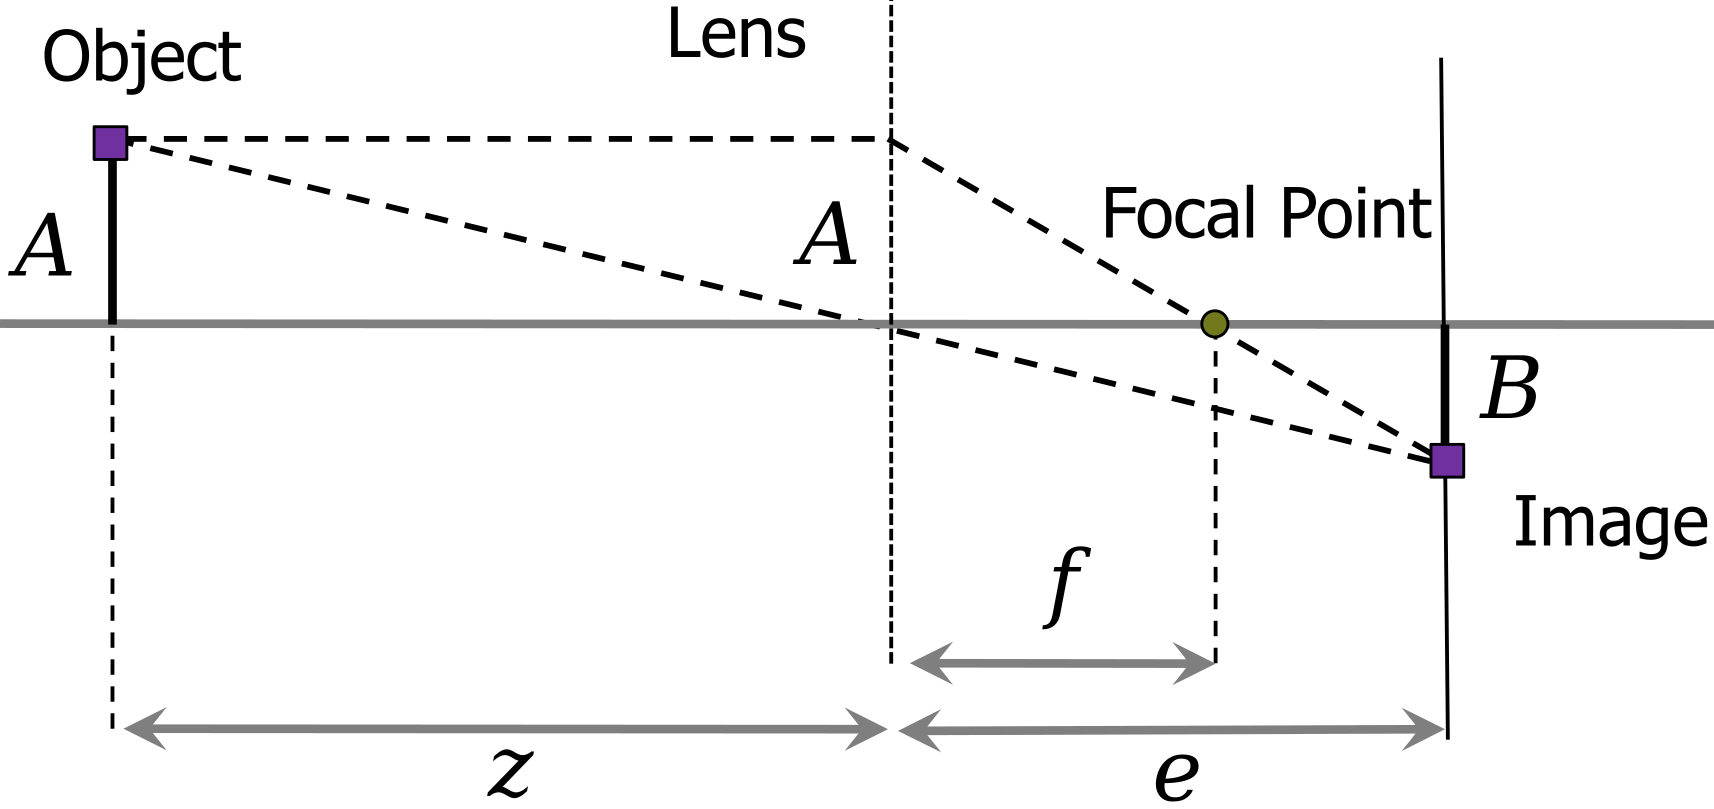
\includegraphics[width=\linewidth]{./Figures/04_ThinLensEquation.png}
    \ides{Pinhole Approximation:} $z \gg f \implies f \approx e$
        \begin{itemize}
            \item I.e. lens is approximated as pinhole at distance $f$ from image plane
            \item If follows that $B = \frac{f}{z}B$
        \end{itemize}
\end{itemize}

\subsubsection{Perspective Camera}
\begin{itemize}
    \item Image plane represented in front of $C$
    \item Camera measures angles and not distances
    \item Project pt $P_W = (x,y,z)$ onto $p_C = (u,v)$ on the image plane
    \ides{Perspective Equations:}\\
        \begin{itemize*}
            \item $x = f \frac{X_c}{Z_C}$
            \item $y = f \frac{Y_c}{Z_C}$
        \end{itemize*}\\
        \begin{itemize*}
            \item $u = u_0 + k x$
            \item $v = v_0 + k y$
            \ides{Scale factor $k$} $[\text{pixels}/\text{meter}]$
        \end{itemize*}
        \begin{itemize}
            \item $\implies \tilde p =
                \begin{bmatrix}
                    \lambda u\\
                    \lambda v\\
                    \lambda
                \end{bmatrix} =
                \underbrace{
                \begin{bmatrix}
                    kf & 0 & u_0\\
                    0 & kf & v_0\\
                    0 & 0 & 1
                \end{bmatrix}}_{K}
                \begin{bmatrix}
                    X_C\\
                    Y_C\\
                    Z_C
                \end{bmatrix}$
        \end{itemize}
    \ides{Intrinsic Parameter $K$:} depending on camera
    \item Rigid Body transformation\\
        $\begin{bmatrix}
            X_C\\
            Y_C\\
            Z_C
        \end{bmatrix}=
        \underbrace{
        \begin{bmatrix}
            r_{11}  & r_{12} & r_{13}\\
            r_{21}  & r_{22} & r_{23}\\
            r_{31}  & r_{32} & r_{33}\\
        \end{bmatrix}}_{R}
        \begin{bmatrix}
        X_W\\
        Y_W\\
        Z_W
        \end{bmatrix} +
        \underbrace{
        \begin{bmatrix}
            t_1\\
            t_2\\
            t_3
        \end{bmatrix}}_{T} = [R \mid T]
        \begin{bmatrix}
            X_W\\
            Y_W\\
            Z_W\\
            1
        \end{bmatrix}$
    \ides{Extrinsic Parameter $[R \mid T]$:} depending on transformation
    \ides{Perspective Projection:} $K[R \mid T]$
    \item $\implies \tilde p =
        \begin{bmatrix}
            \lambda u\\
            \lambda v\\
            \lambda
        \end{bmatrix} = K[R \mid T]
        \begin{bmatrix}
            X_W\\
            Y_W\\
            Z_W\\
            1
        \end{bmatrix}$
    \ides{Barrel Distortion}
        \begin{itemize}
            \item Straight lines get bend
            \ides{Barrel Distortion:} Image gets ``round''
            \ides{Pincusion Distortion:} Corners pulled out
            \item Model:
                $\begin{bmatrix}
                    u_d\\
                    v_d
                \end{bmatrix} = (1 + k_1 r^2)
                \begin{bmatrix}
                    u - u_0\\
                    v - v_0
                \end{bmatrix} +
                \begin{bmatrix}
                    u_0\\
                    v_0
                \end{bmatrix}$
                \begin{itemize}
                    \ides{Distortion Parameter $\mathbf{k_1}$:} Intrinsic parameter
                    \item $r^2 = (u - u_0)^2 + (v - v_0)^2$
                \end{itemize}
        \end{itemize}
\end{itemize}

\subsubsection{Omnidirectional Camera}
\begin{itemize}
    \ides{Dioptric:}
        \begin{itemize*}
            \item System of lenses
            \item $\sim 180^\circ$ FOV
        \end{itemize*}
    \ides{Catadioptric:}
        \begin{itemize*}
            \item Combination of lens and mirrors
            \item $> 180^\circ$ FOV
            \item Greatly distorted (can be removed depending on mirror)
        \end{itemize*}
        \begin{itemize}
            \ides{Central Camera:} Mirror shaped that all incoming rays have same \textit{single effective viewpoint}
                \begin{itemize}
                    \ides Correct mirror placement is important
                    \ipro Unwarping into perspective image possible
                    \ipro Can convert points in the image to spherical vectors
                    \ipro Can apply standard algorithms
                \end{itemize}
        \end{itemize}
    \ides{Polydioptric:}
        \begin{itemize*}
            \item Multiple cameras
            \item $\sim 360^\circ$ FOV
        \end{itemize*}
\end{itemize}

\subsubsection{Camera Calibration}
\begin{itemize}
    \item Determine intrinsic (and extrinsic) camera parameters
    \item Done using least-square method
\end{itemize}

\subsubsection{Stereo Vision}
\begin{itemize}
    \item Obtain depth information from two cameras with know relative position
    \item Cameras need to be calibrated
    \item Calculating depth $Z_P$ of point $P_W$ (distance to $P_W$)
    \ides{Baseline $\mathbf{b}$:} Distance between the two cameras
    \ides{Disparity:} Difference in image location of the projection of a 3D point on the two image panes: $u_l - u_r$
    \item Two identical cameras aligned on $x$
        \begin{itemize}
            \item $Z_P = \frac{bf}{u_l - u_r}$
        \end{itemize}
    \item Two identical cameras in different Coordinate Systems
        \begin{itemize}
            \item $C_r$ is a rigid body transformation of $C_l$\\
            \item Triangulation
            \begin{itemize*}
                \item $\tilde p_l = \lambda_l
                    \begin{bmatrix}
                        u_l\\
                        v_l\\
                        1
                    \end{bmatrix} = K_l
                    \begin{bmatrix}
                        X_W\\
                        Y_W\\
                        Z_W
                    \end{bmatrix}$
                \item $\tilde p_r = \lambda_r
                    \begin{bmatrix}
                        u_r\\
                        v_r\\
                        1
                    \end{bmatrix} = K_r R
                    \begin{bmatrix}
                        X_W\\
                        Y_W\\
                        Z_W
                    \end{bmatrix} + T$
            \end{itemize*}
        \end{itemize}
    \ides{Disparity Map}
        \begin{itemize}
            \item Compute disparity for corresponding points of every pixel
            \item Can compute the depth from it and reconstruct 3D scene
        \end{itemize}
\end{itemize}

\subsubsection{Correspondence Search}
\begin{itemize}
    \item Identify corresponding points in two images of the same scene
    \item Measure similarity of two pts using a similarity measurement
    \ides{Epipolar Plane:} Spanned by $C_l$, $C_r$ and some pt $P_W$
    \ides{Epipolar Line:} Projection of the ray from one camera through points in the other camera
    \ides{Epipole:} Projection of other camera in image plane
        \begin{itemize*}
            \item All epipolar lines go through it
        \end{itemize*}
    \ides{Epipolar Constraint:} Correspond of pt of left images lies on the epipolar line of the right image
    \ides{Epipolar Rectification:} Transform both images to make epipolar lines collinear and parallel:
        \begin{itemize*}
            \item[1)] Remove radial distortion
            \item[2)] \textbf{Warping:} Reprojection of both images to same plane
        \end{itemize*}
\end{itemize}

\subsubsection{Structure from Motion (SfM)}
\begin{itemize}
    \item Given corresponding image points $\{(u_1^i, v_1^i), (u_2^i, v_2^i)\}$, recover:
        \begin{itemize*}
            \item 3D location $P_i$ of all $n$ pts
            \item Relative pose of right camera $R, T$
            \item Camera intrinsic $K$ (optionally)
        \end{itemize*}
    \item Assume $K$ is known
    \ides{Knowns:} $4n$: $n$ correspondences
    \ides{Unknowns:} $5 + 3n$: rotation ($3$), translation ($2$, since scale cannot be recovered), $n$ 3D pts ($3n$)
    \item Solution exists iff $4n \ge 5 + 3n \implies n \ge 5$
    \ides{Crossp.:} $a \times b =
        \begin{bmatrix}
            0 & -a_z & a_y\\
            a_z & 0 & -a_x\\
            -a_y & a_x & 0
        \end{bmatrix}
        \begin{bmatrix}
            b_x\\
            b_y\\
            b_z
        \end{bmatrix} = [a]_\times b$
    \ides{Epipolar Constraint:} $p_2^T E p_1 = 0$
    \ides{Essential Matrix:} $E = [T]_\times R$
        \begin{itemize}
            \item Computed with $\ge 5$ correspondences
            \item Can be decomposed into $R$ and $T$
        \end{itemize}
    \ides{Normalized Img Coordinates:} $p = [\bar u, \bar v, 1]^\transpose = K^{-1}[u, v, 1]^\transpose$
    \ides{8-pt Algorithm}
        \begin{itemize*}
            \item Algorithm to compute essential matrix
            \item Uses $\ge 8$ pts
        \end{itemize*}
        \begin{itemize}
            \item $p_2^\transpose E p_1 = [\bar u_2, \bar v_2, 1]
                \begin{bmatrix}
                    e_11 & e_12 & e_13\\
                    e_21 & e_22 & e_23\\
                    e_31 & e_32 & e_33
                \end{bmatrix}
                \begin{bmatrix}
                    \bar u_1\\
                    \bar v_1\\
                    1
                \end{bmatrix} = 0$
            \item $\underbrace{[u_2u_1, u_2v_1, u_2, v_2u_1, v_2v_1, v_2, u_1, v_1, 1]}_{Q: \text{known}}\underbrace{[e_{11}, e_{12}, \dots, e_{33}]}_{\text{unknown}} = 0$
            \item For $8$ non-coplanar pts, unique solution is given by the EV of $Q$ corresponding to the smallest Eigenvalue
        \end{itemize}
\end{itemize}
